\documentclass[a4paper, 12pt,oneside]{article} 
%\documentclass[a4paper, 12pt,oneside,draft]{article} 

\usepackage{preamble}
\usepackage{bm}
%--------------------- ACTUAL FILE ---------------------- %
\begin{document} 
	\begin{center}
	    \Large
	    \textbf{Project 6 : Sea level extremes in Venice}
	    \vspace{0.4cm}
	    \large
        
	    Author : Tara Fjellman \\
	    \small{Spring 2024}
	\end{center}
    \section{Introduction}
    The city of Venice and its lagoonal ecosystem are vulnerable to changes in sea levels. The occurrences of high tides (aqua alta) has an increasing trend, usually attributed to global warming. Due to Venice's unique environmental and cultural significance, a project called MOSE (Modulo Sperimentale Elettromeccanico) was initiated to safeguard the Venetian Lagoon from flooding. According to MOSE, water levels reaching or exceeding 140 cm are considered extreme high waters$^{[1]}$ In this report, we analyze the sea levels in Venice and assess the severity of extreme events. We use a GEV model to fit the data and compute its associated  return levels. We then compare these to the extreme events that occurred between 2013 and 2023. The goal is to assess the significance of the severity increase associated to these events. 
    \section{Data exploration}
        \subsection{Data description}
        For our analysis we mainly use the \texttt{venice90} dataset available in the \texttt{VGAM} package (in \texttt{R}). This dataset contains hourly sea levels greater than 90 cm from 1940 to 2009. The data are declustered to ensure each value is at least 24 hours apart, in the effort to ensure data independence. We also use the (2013 to 2023 part of the) dataset of extreme events that can be found on the MOSE Wikipedia page. These events correspond to high tides exceeding 140 cm.
        \subsection{Maxima evolution}
        To start the analysis, we first consider the yearly maxima of the sea levels. The yearly maxima are plotted in \ref{fig:data-series}. The red points represent the yearly maxima. The data seem to show an increasing trend in the yearly maxima, which is consistent with the general trend of increasing sea levels. There is also an event in 1966 where the yearly maximum was particularly high, exceeding 190 cm.
        \begin{figure}[h!]
            \centering
            \vspace{0em}
            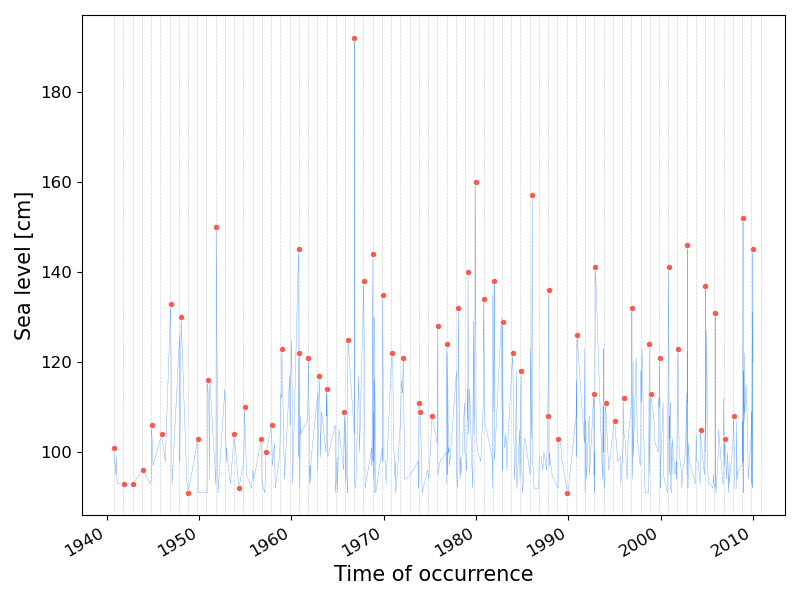
\includegraphics[width=.7\textwidth]{data-series}
            \caption{Data from the \emph{\texttt{venice90}} dataset. The red points represent the yearly maxima.}
            \label{fig:data-series}
        \end{figure}
        To confirm the initial observation of an increasing trend, we fit a gamma GLM  (and log link function) to the yearly maxima. We chose a gamma GLM as the distribution of the maxima is positive and skewed. The fitted model is shown in \ref{fig:glm-plot}. The model confirms the increasing trend in the yearly maxima. The model however does not capture well the extreme events, such as the one in 1966. This is expected since the Gamma distribution is not well suited to model extreme values. Problems are particularly noticeable when considering the extreme data points that occurred between 2013 and 2023 (from the MOSE dataset).
        \begin{figure}[h!]
            \centering
            \vspace{0em}
            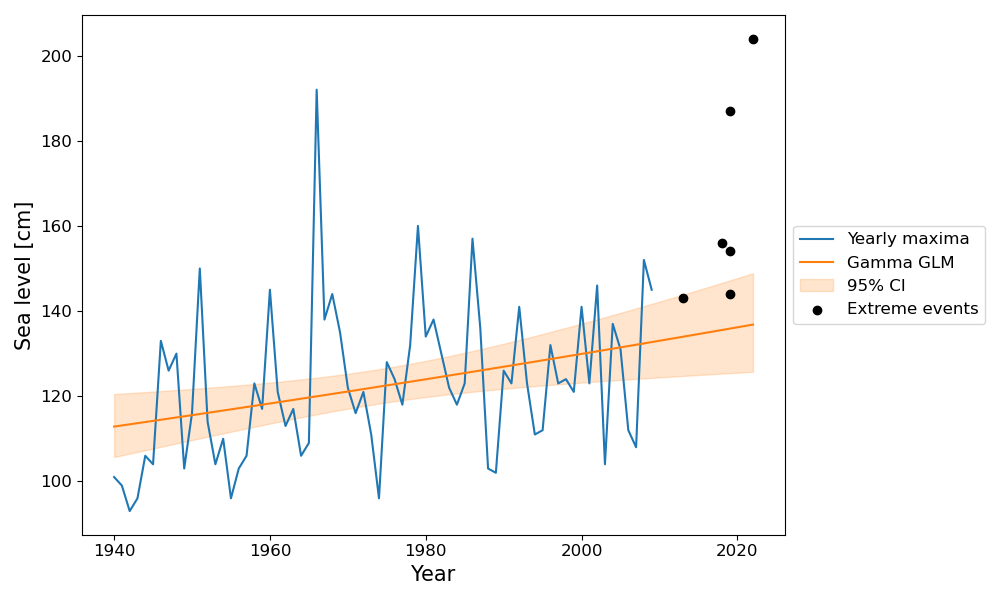
\includegraphics[width=.75\textwidth]{glm-plot}
            \caption{Gamma GLM fit of the yearly maxima. Extreme events that occurred between 2013 and 2023 are also included.}
            \label{fig:glm-plot}
        \end{figure}
        In the next section, we try and tackle this by fitting a GEV model to the data and computing the associated return levels. This should be more suited to model extreme values and will make it easier to assess weather the severity in extreme values observed between 2013 and 2023 is significant.
    \section{GEV model}
        \subsection{Model selection}
        When fitting a GEV to data that has a time-dependent distribution, one can consider many different models. In this section we compare the adequacy of three different models. The first assumes that all parameters are constant in time, the second allows the location parameter to vary linearly in time, while the third allows both the location and the scale parameter to vary in time. The reason for which we did not consider a shape parameter that varies in time is that to detect a time-varying shape parameter, one would need a lot of data. Already in the current set up, the estimate of the shape parameter was quite unstable. 

        To select the best model we use LRTs between nested models. We first test for significance of the time-varying location parameter against the constant model, and then test for significance of the time-varying scale parameter against the time-varying location parameter model. The results are respectively $p=6.51\times 10^{-4}$ and $p=3.45\times 10^{-1}$. this suggests that the time-varying location model is significantly better than the constant model, while the time-varying scale model is not significantly better than the time-varying location model. We thus choose the time-varying location model as our final model.
        \subsection{Model diagnostics}
        In this section we present the diagnostic plots of the selected model. The QQ plot is shown in the left panel of \ref{fig:diagnostic-plot}. The KDE of the data and the PDF of the model are shown in the right panel. The plotted PDF is a mixture of the fitted GEV evaluated at each year, as within out model the maxima $x_y$ associated to a given year $y$ follows the $f_{\mu(t_y),\sigma,\xi}(x_y)$ distribution.
        \begin{figure}[h!]
            \centering
            \vspace{0em}
            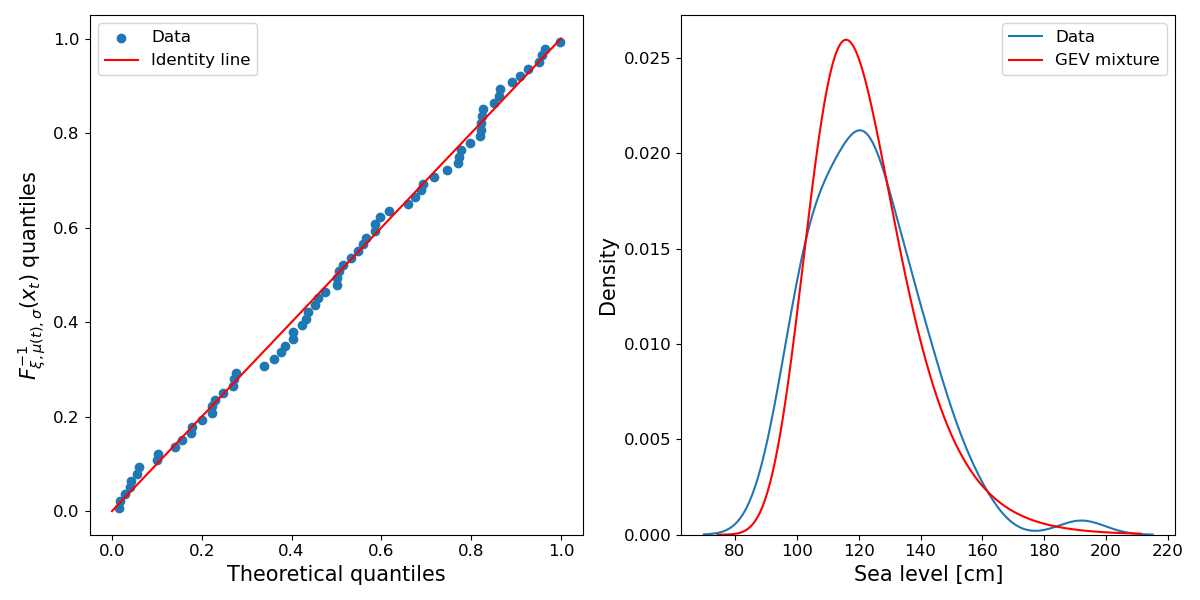
\includegraphics[width=\textwidth]{diagnostic-plot}
            \caption{Diagnostic plots of the model with time-varying mu and constant other parameters. Left : QQ plot. Right : KDE of the data and PDF of the model (mixture composed of the fitted GEV evaluated at each year).}
            \label{fig:diagnostic-plot}
        \end{figure}
        The model seems to fit the data quite well. Indeed the points in the QQ plot align with the identity line. The plot of the KDE and the PDF allows us to carry the analysis deeper. The model seems to capture well the general shape of the data. However, the KDE presents a slight bimodality that is not accounted for by the model. This is probably an artificial feature that is due to the limited amount of data. Indeed, as time advances, we expect events between the outlier of 1996 and the other to occur and cancel the bimodality.  
    \section{Risk analysis}
    In this section we present the 14 and 30 year return levels of the GEV model and compare them to the extreme events that occurred between 2013 and 2023. The goal is to asses the significance of the severity increase associated to them. The relevant plot is shown in \ref{fig:risk-analysis-plot}.
    \begin{figure}[h!]
        \centering
        \vspace{0em}
        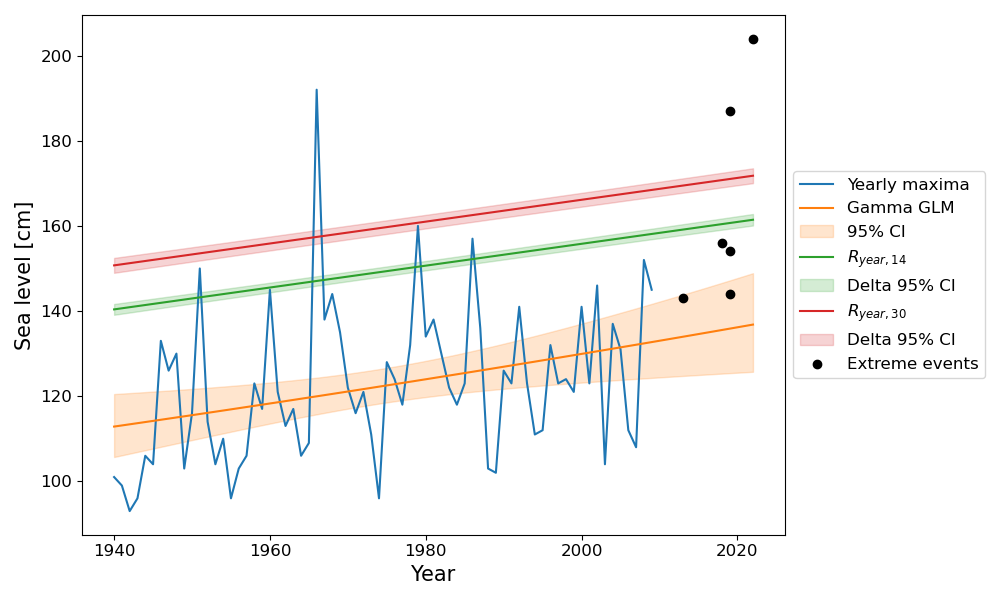
\includegraphics[width=.75\textwidth]{risk-analysis-plot}
        \caption{Gamma GLM fit of the yearly maxima and to the 14 \& 30 year return levels. Extreme events that occurred between 2013 and 2023 are also included.}
        \label{fig:risk-analysis-plot}
    \end{figure}
    Looking at the figure, we see that some of two of the extreme events that occurred between 2013 and 2023 are far above both the 14 and 30 year return levels. These return levels seem however consistent with the training set, as only 4 (resp. 2) out of the 69 years are associated with maxima greater than the 14 (resp. 30) year return level. This suggests that the increase in severity of these events is greatly significant. 
    \section{Conclusion}
    Summary of findings from the data analysis and predictions
    In this report we analyzed the sea levels in Venice and assessed the severity of extreme events. We used a GEV model to fit the data and compute its associated return levels. We then compared these to the extreme events that occurred between 2013 and 2023. The results suggest that the severity increase associated to these events is significant.
    It therefore seems that the MOSE project is more than justified in its efforts to safeguard the Venetian Lagoon from flooding. Further monitoring of the sea levels is however necessary to ensure the project remains effective. Some uncertainty on the sufficiency of the MOSE project by 2100 has indeed already been cast by the IPCC in 2019$^{[2]}$.
    \section{Nota Bene}
    The goal was initially to compute the confidence intervals of the return levels in two different ways : using the delta method and using parametric bootstrap. Both theses methods were actually coded and can be found in the submitted scripts. The bootstrap method was however not used in this report due to a technical problem. Indeed, no method was found for the likelihood maximisation of the GEV model to be stable enough as to converge for the large number of bootstrap datasets. 

    We expect the parametric bootstrap to have better accounted for the limited amount of data.  
    \section*{Acknowledgements}
    I thank Laurent Brugnard and Rayan Harfouche for discussions during and outside the exercise sessions. I also acknowledge I provided Rayan Harfouche with a minimal version of the GEV log-likelihood maximisation code as a starting point for his own implementation. I allowed myself to do this since the implementation itself was not meant to be part of the exercise.  
    \section*{References}
    [1] ‘Wikiwand - MOSE’, Wikiwand. Accessed: May 14, 2024. [Online]. Available: https://www.wikiwand.com/en/MOSE

    [2] C. Harlan and S. Pitrelli, ‘How Venice’s plan to protect itself from flooding became a disaster in itself’, Washington Post, Nov. 19, 2019. Accessed: May 14, 2024. [Online]. Available: https://www.washingtonpost.com/world/europe/how-venices-plan-to-protect\newline
    -itself-from-flooding-became-a-disaster-in-itself/2019/11/19/7e1fe494-09a8-11ea-8054-\newline
    289aef6e38a3\_story.html
\end{document}